\documentclass[10pt,letterpaper]{article}

\usepackage{cvpr}
\usepackage{times}
\usepackage{epsfig}
\usepackage{graphicx}
\usepackage{amsmath}
\usepackage{amssymb}
\usepackage{kotex}
\usepackage{pifont}

\newcommand*\OK{\checkmark}
\newcommand*\BOLDOK{\ding{51}}

% Include other packages here, before hyperref.

% If you comment hyperref and then uncomment it, you should delete
% egpaper.aux before re-running latex.  (Or just hit 'q' on the first latex
% run, let it finish, and you should be clear).
\usepackage[breaklinks=true,bookmarks=false]{hyperref}

\cvprfinalcopy % *** Uncomment this line for the final submission

\def\cvprPaperID{****} % *** Enter the CVPR Paper ID here
\def\httilde{\mbox{\tt\raisebox{-.5ex}{\symbol{126}}}}

% Pages are numbered in submission mode, and unnumbered in camera-ready
%\ifcvprfinal\pagestyle{empty}\fi
\setcounter{page}{1}
\begin{document}

%%%%%%%%% TITLE
\title{Final Project. CAPTCHA Image Recognition using CNN and LSTM}

\author{Sangjun Son\\
Seoul National University\\
Department of Computer Science and Engineering\\
{\tt\small lucetre@snu.ac.kr}
}

\maketitle

\section{Introduction}


Everyone hates CAPTCHAs — those annoying images that contain text you have to type in before you can access a website \cite{captcha}. A CAPTCHA (an acronym for "Completely Automated Public Turing test to tell Computers and Humans Apart") is a type of challenge–response test used in computing to determine whether or not the user is human \cite{recaptcha}. It is to prevent computers from automatically filling out forms by verifying that you are not a robot. But with the rise of deep learning and computer vision, decoding CAPTCHA seems to be possible and some of those systems are even more better than human.

Given an image, how can we recognize characters from the CAPTCHA image? Since each CAPTCHA image has a variable length of characters, considering length will be a significant work while training through deep neural networks. If we can split the image apart so that that each letter is a separate image, remaining work is just to train the neural network to recognize a single letter at a time\cite{captcha}.

\begin{center}
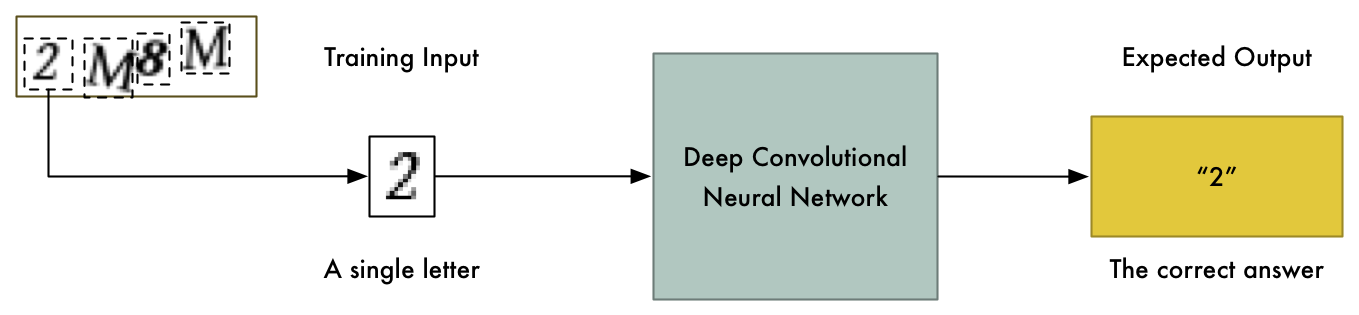
\includegraphics[width=1\linewidth]{./overview.png}
\end{center}

We've trained our network with 10,000 training examples whose lengths are in 2 $\sim$ 5 and tested with 1,000 test images of length 2 $\sim$ 7. Due to several parameters consisting the ensemble model of CNN and LSTM, we've conduct various experiments. After several experiments, we've found the best set of hyper-parameters that make our model perform more accurately and even faster.


%-------------------------------------------------------------------------
\section{Related Works}

CATCHA recognition is one part of temporal pattern recognition projects. Simiarly, there are numerous examples like image captioning, speech recognition, part-of-speech tagging. Using ResNet and LSTM modules, which are the representatives of CNN and RNN methods, we can extract useful features from an image and continuously learning them over time.

%-------------------------------------------------------------------------
\section{Proposed Method}
This section describes overall flows of our proposed method, \texttt{BetterNet+LSTM}. Feature extraction and learning the temporal patterns are the key concepts of our model.

\begin{center}
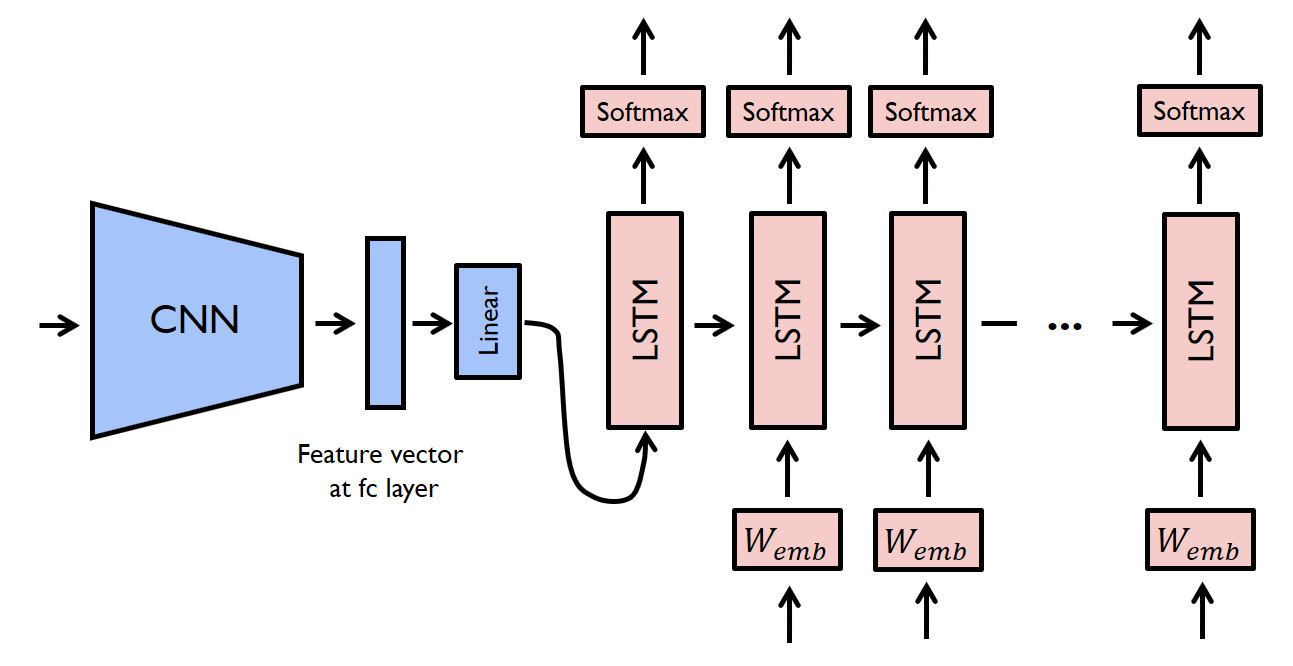
\includegraphics[width=0.7\linewidth]{./model.jpg}
\end{center}

\subsection{Feature extraction by BetterNet}
Since image vectors contain lots of information, we have to extract meaningful features. Pre-training inputs through ResNet, we


\subsection{Learning temporal patterns by LSTM}
The pretrained CNN extracts the feature vector from a given input image. The feature vector is linearly transformed to have the same dimension as the input dimension of the LSTM network.
Using these source and target sequences and the feature vector, the LSTM decoder is trained as a language model conditioned on the feature vector \cite{image-captioning}.

%-------------------------------------------------------------------------
\section{Empirical Analysis}

Here we describes how we came up with \texttt{jerk8vel8iter50} model. And this is the table of comparison in 1-iteration trained models in aspect of test accuracy.

{\centering
\begin{tabular}{ p{3cm}| ccc | c}
 \hline
 Model Name & jerk $j$ & acc $a$ & vel $\alpha$ & Accuracy \\
 \hline
 \texttt{jerk8} & \OK & & & 50.81\% \\
 \texttt{acc8} & & \OK & & 35.24\% \\
 \texttt{vel8} & & & \OK & 60.65\% \\
 \texttt{acc8vel8} & & \OK & \OK & 78.68\% \\
 \texttt{jerk8acc8} & \OK & \OK & & 40.16\% \\
 \texttt{jerk2vel8} & \OK & & \OK & 63.93\% \\
 \texttt{jerk4vel8} & \OK & & \OK & 79.50\% \\
 \texttt{\textbf{jerk8vel8}} & \BOLDOK & & \BOLDOK & \textbf{84.42\%} \\
 \texttt{jerk8acc2vel8} & \OK & \OK & \OK & 63.11\% \\
 \hline
\end{tabular}
}

\subsection{Feature Metric Approach}
When deciding what feature metric would be suitable, we've compared many different models trained for 1 iteration and chose the metric of the model with best test accuracy. From the table above, we've found angular velocity data measured from gyro sensor and jerk data were the significant classifiers in this approach. In conclusion, using \texttt{jerk8vel8} model was the best.

\subsection{Model Complexity Approach}
When we construct HMM model with too many states, there can be over-fitting issues that our model only estimates trained data accurately but not test data. By differing number of observation states, we've found out the model having the best complexity would also be \texttt{jerk8vel8}.

%-------------------------------------------------------------------------
\section{Conclusion}
Understanding human behaviour using sensor models needs temporally learning models since the dataset is also time-serial. Many other works determining human action recognition uses RNN models like LSTM, probabilistic models like particle filter or in hybrid. We've constructed HMM model simply learning the observation patterns from HAR dataset produced by Jorge L, \etal.

Dataset includes 1,214 instances of 12 human actions and provides acceleration and angular velocity vectors. Feature extraction in acceleration and angular velocity vector was to splitting its direction into 8 sections, numbered them and use to define observation states. With empirical approaches, we've figured out \texttt{jerk8vel8} having appropriate model complexity and high test accuracy as well.

We've trained this model with maximum training iteration of 50 and \texttt{jerk8vel8iter50} showed remarkable performance of 92.62\% as the test accuracy and 24623.64s as the training time. In future works, we'll improve our model with numerous instances created from more experiments and use other additional sensors to extract various states features.

\begin{thebibliography}{9}

\bibitem{captcha} 
Adam Geitgey, ``How to break a CAPTCHA system in 15 minutes with Machine Learning", Dec. 2017

\bibitem{recaptcha} 
Adam Geitgey, ``The reCAPTCHA Project – Carnegie Mellon University CyLab". {\textit{www.cylab.cmu.edu. Archived}}, Jan. 2017

\bibitem{image-captioning} 
yunjey, ``Image Captioning", {\textit{GitHub pytorch-tutorial}}, Nov. 2018

\bibitem{biology} 
Byung-Jun Yoon, 
``Hidden Markov Models and their Applications in Biological Sequence Analysis"

\bibitem{speechrecognition} 
M. Gales and S. Young
``The Application of Hidden Markov Models in Speech Recognition".
{\textit{Foundations and Trends in Signal Processing, Vol.1, No.3}, 2007}

\bibitem{hapt}
Jorge L. Reyes-Ortiz, Davide Anguita, Alessandro Ghio, Luca Oneto and Xavier Parra,
``Smartphone-Based Recognition of Human Activities and Postural Transitions Data Set"
, 2015

\bibitem{haptpaper}
Jorge L, \etal
``Human Activity Recognition on Smartphones with Awareness of Basic Activities and Postural Transitions"
{\textit{ICANN 2014, LNCS 8681, pp.177–185}, 2014}

\bibitem{monitoring}
Rubén San-Segundo, Julián David Echeverry-Correa, Christian Salamea, José Manuel Pardo
``Human activity monitoring based on hidden Markov models using a smartphone"
{\textit{IEEE Instrumentation and Measurement Magazine}, 2016}

\bibitem{hmm}
Daniel Jurafsky and James H. Martin.
``Hidden Markov Models"
{\textit{Speech and Language Processing}, 2019}

\bibitem{jerkwiki} 
Wikipedia, Jerk (physics)

\bibitem{sklearn} 
API Documentation of sklearn, model selection, train test split


\end{thebibliography}
% [8] API Documentation of hmmlearn.MultinomialHMM (https://hmmlearn.readthedocs.io/en/latest/api.html#multinomialhmm)

\end{document}
